
Urban areas typically do not offer classic emergency landing sites such as unpopulated open fields requiring a planner to consider unconventional yet safe alternatives. We propose flat building rooftops as viable urgent landing sites for small UAS.  During landing site selection, a map-based planner must be able to assess landing site risk posed to the aircraft and bystanders at touchdown. The UAS may pose risk to people and property it overflies enroute, so the planner must also assess path risk once the landing flight plan is known.  Landing site and path risk together offer an estimate of \emph{total risk}.

Map data used for emergency landing planning must have high integrity and low-latency access to support timely decision making. This chapter proposes an offline data processing pipeline and online multi-objective, multi-goal landing planner that enable a UAS to minimize total risk when a nearby emergency landing is required. GIS data sources are processed to generate an on-board landing site database and occupancy map as shown in Figure \ref{fig:ch5_overview_processing}.  The multi-goal onboard emergency landing planner explores available ground and rooftop landing sites likely to minimize overall total risk while greedily pruning options known to have higher risk.   Pareto fronts over landing site and path risk are generated for three urban regions: Witten, Germany; Ann Arbor, Michigan; and mid-town Manhattan in New York City. We statistically analyze results with respect to availability and quality of landing sites as well as execution time of the map-based planner.


\begin{figure}[!t]
    \centering
    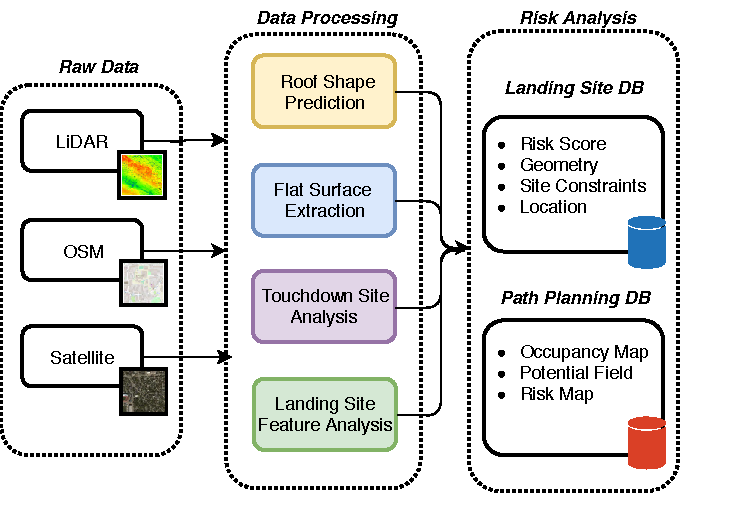
\includegraphics[clip, trim=0.0cm 0cm 0cm 0cm, width=0.6\linewidth]{chapter_5_mapping/imgs/data_preprocessing-Page-1.pdf}
    \caption{Data processing pipeline to construct landing site and occupancy map databases with risk values.}
    \label{fig:ch5_overview_processing}
\end{figure}


\paragraph{Landing Site Selection}
A set of candidate landing sites are generated within a radial footprint $R$
\begin{align}
    \mathcal{S}_{ls} = \{ l_i, \ldots, l_n \}
\end{align}
where each $l_i$ refers to a landing site with properties
\begin{align}
    l_i = \{ \mathbf{c},\; r_{l}, \;r_{p} \} \\
    \mathbf{c} \in \mathbb{R}^3 \\
    r_{l}, r_{p}  \in \mathbb{R} %\in [0,1]
\end{align}
where $\mathbf{c}$ is landing site location in a Cartesian reference frame, $r_{l}$ is landing site risk, and $r_{p}$ is path risk. Landing site risk is calculated offline and represents the risk intrinsic to touching down at that landing site. Path risk must be calculated online and accounts for the path distance and proximity to obstacles. A linear weighting scheme between the objectives is proposed below for each landing site $l_i \in \mathcal{S}_{ls} $:
\begin{equation}\label{eq:total_risk}
    r_{t} = w_l \cdot r_{l} + w_p \cdot r_{p}
\end{equation}
where $r_{t}$ refers to the total risk and $w_l$ and $w_p$ are weights for landing site risk and path risk, respectively. The optimal landing site can then be found by solving the optimization problem shown in Eq. \ref{eq:optimization}.
\begin{equation}
    l_{i^*} = \argminA_{l_i \; \in \; \mathcal{S}_{ls}} \; r_{t}\label{eq:optimization}
\end{equation}

A key insight into our multi-goal planner is that the minimum total risk $r_{t,min}$ of all landing sites can be calculated without computationally expensive path planning by using distance heuristics. The multi-goal planner can then prioritize searching for landing sites by lowest $r_{t,min}$ and halt search once a landing site's true total risk is less than all other sites' minimum total risk. 
% something I want to do later is paralleize this

\paragraph{Results}

An example case study in Witten is shown in Figure \ref{fig:ch5_ny_map1}. The position of the UAS is indicated by the green marker with nearby landing sites shown in color. Landing site risk is colorized from low (yellow) to high (dark orange) risk, with associated touchdown sites marked as blue circles. The lowest risk landing sites are ranked and marked with blue numbered icons. Our planner's chosen landing site is marked in red; this site balances landing site and path risk. Figure \ref{fig:ch5_ny_pareto} shows a Pareto plot demonstrating the trade off between landing site risk and path risk. Each purple dot represents risk for a landing site and its risk-optimal associated path, while the red dot signifies the planner's choice which minimizes total weighted risk. The green Pareto front connects the risk-optimal landing sites with respect to landing site and path risk.
% To generate these plots, collision-free paths to \textit{all} landing sites were generated, providing their actual path risk. 
% The $A^{*}$ path planning algorithm is used to search through occupancy maps to determine trajectories to landing sites and their associated path risk, $r_p$.
% Publicly available GIS data sources from the cities of Witten, Ann Arbor, and New York were processed to create risk-evaluated landing site databases and occupancy maps for path planning as outlined in Figure \ref{fig:ch5_overview_processing}. 

\begin{figure}
    \centering
    \begin{subfigure}[b]{0.44\linewidth}
        % \centering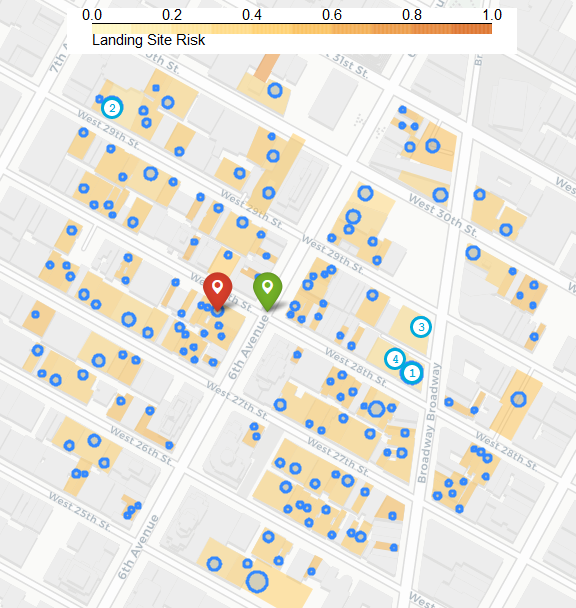
\includegraphics[clip, width=155pt, height=130pt]{chapter_5_mapping/imgs/newyork_scenario_1.png}
        \centering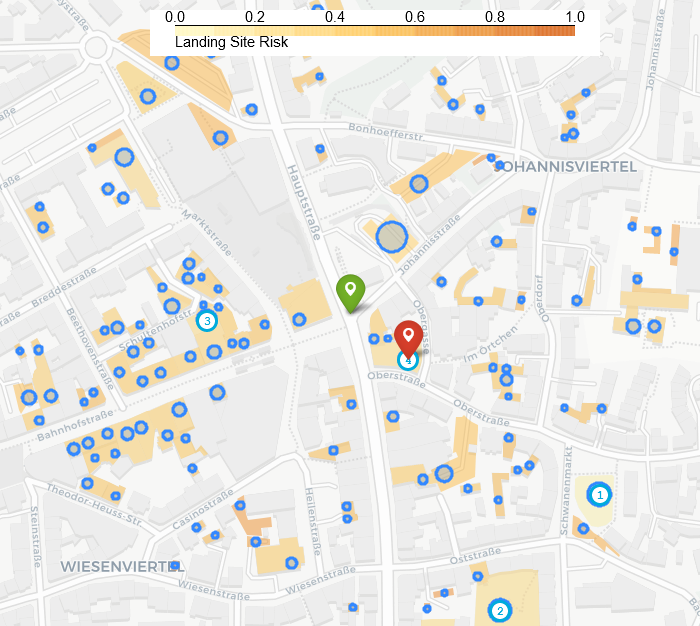
\includegraphics[clip, width=\linewidth, height=170pt]{chapter_5_mapping/imgs/witten_scenario_1.png}
        \caption{\label{fig:ch5_ny_map1}}
    \end{subfigure}
    \begin{subfigure}[b]{0.49\linewidth}
        % \centering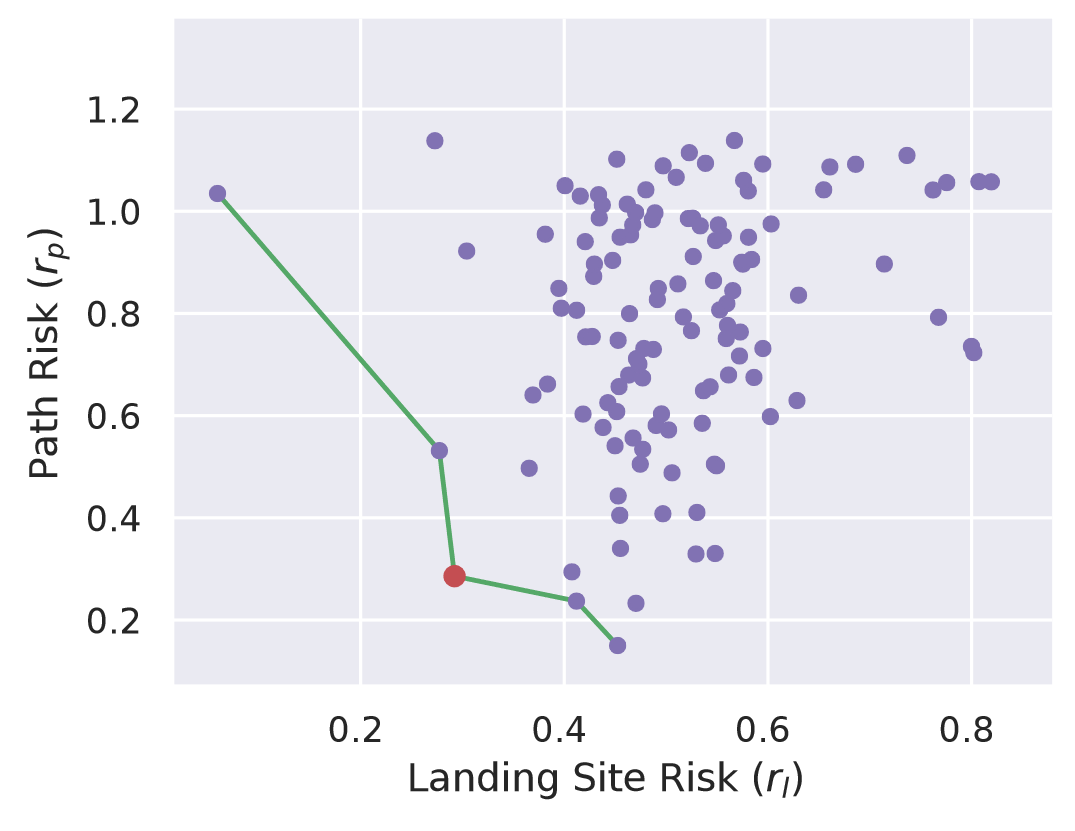
\includegraphics[clip, width=155pt, height=130pt]{chapter_5_mapping/imgs/PaertoFront.png}
        \centering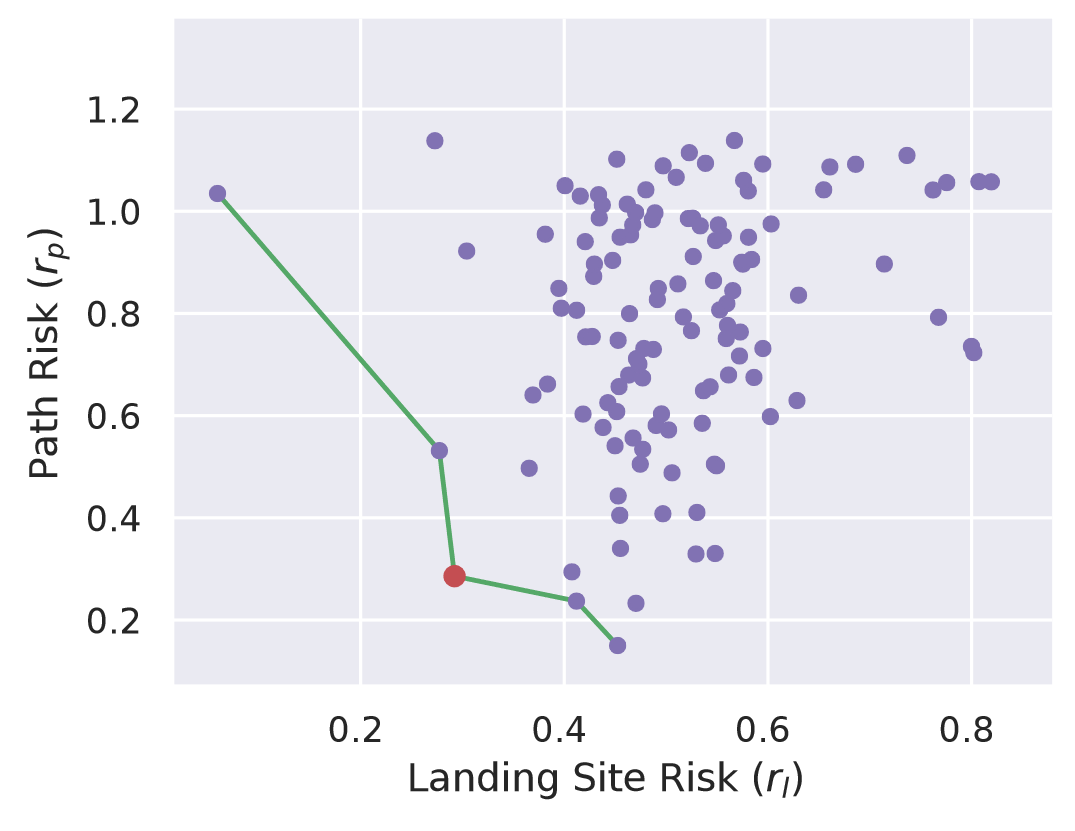
\includegraphics[clip, width=\linewidth, height=170pt]{chapter_5_mapping/imgs/PaertoFront.png}
        \caption{\label{fig:ch5_ny_pareto}}
    \end{subfigure}
    \caption{Urgent landing scenario in Manhattan New York. (\subref{fig:ch5_ny_map1}) Map of risk-evaluated landing sites (\subref{fig:ch5_ny_pareto}). Each purple dots represents a landing site and its associated path, while the red dot signifies the planner's choice that minimizes total weighted risk. }
    \label{fig:ch5_landing_site_selection}
\end{figure}


% \section{}

\paragraph{Conclusion}
This chapter demonstrates the use of nearby flat rooftops to augment traditional emergency landing sites such as parks and fields. Suitable rooftop surfaces are found by processing offline GIS data with roof shape identification and flat surface extraction with clear flat surfaces ultimately represented as polygons. Touchdown points for all terrain and rooftop surfaces are found by optimizing over distance to obstacles and calculating landing site risk. Landing site databases and 3D risk maps were generated for three diverse cities with results presented from six case studies with one example presented in this chapter summary. The multi-goal landing path planner minimizes a weighted sum of landing site and path risk for the UAS. A full description of all methods, risk models, and results can be found in our full paper \cite{castagno_map-based_2021}.